\documentclass{article}

\usepackage{fontspec}   %加這個就可以設定字體
\usepackage{xeCJK}       %讓中英文字體分開設置
\setCJKmainfont{標楷體} %設定中文為系統上的字型,而英文不去更動,使用原TeX字型
\setmainfont{Calibri} % 設定英文字型
\XeTeXlinebreaklocale "zh"             %這兩行一定要加,中文才能自動換行
\XeTeXlinebreakskip = 0pt plus 1pt     %這兩行一定要加,中文才能自動換行

\usepackage{titling}
\setlength{\droptitle}{-12em} % 將標題移動至頁面的上面


\title{第二章、Duckietown電腦端之環境架設}

\author{林哲民}
\date{} %不要日期

\begin{document}
\maketitle

\section{應用之工具安裝及網路架設}

我們需要一個可以直接開發Duckietown之環境,因此我們選擇在電腦上使用一些工具作為Duckietown之開發環境,如此可以省去在機器之使用者介面上之額外花費。
\subsection{虛擬電腦軟體:VirtualBox}

Duckietown之程式運作所使用的系統作業軟體是Linux Ubuntu 14.04,考慮到現今大多數人都使用Windows、IOS系統,因此我們選擇以虛擬電腦軟體為主體來進行Duckietown之運作環境。
\\VirtualBox是一套免費開放原始碼的虛擬電腦軟體,讓你在原有的系統架構下再建立出一台或是多台的新電腦。且可以在虛擬電腦裡安裝不同的作業系統,或是進行軟體測試,最重要的是在虛擬電腦裡所進行的動作皆不會影響或干擾到原有的電腦。接下來,我們會教學如何設定VirtualBox。
\\
\\步驟一、下載VirtualBox
\\官方網站(https://www.virtualbox.org/wiki/Downloads)有提供載點根據你筆電的作業系統進行下載。

\begin{figure}[htp]
    \begin{center}
        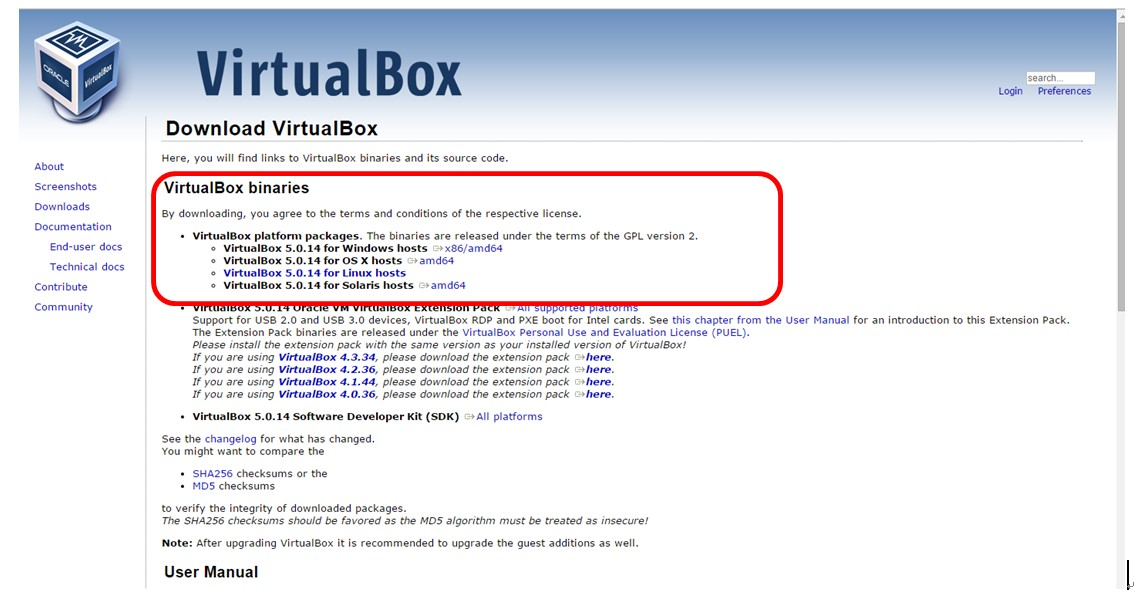
\includegraphics[width=250pt]{pic/圖片1.jpg}
    \end{center}
\end{figure}
已知有支援的作業系統:Windows7/10 64 bit; Ubuntu 14.04.3 32/64 bit; MacBook Pro (mid-2014)
\\步驟二、取得VirtualBox映像檔
\\針對Duckietown,我們已經準備相對應之映像檔供學生使用,連結如下:
robotic-vision-v2 (in progress):
https://drive.google.com/open?id=0B6vRmsV8B-ToQTJ3UmRzVHIyYXc
此映像檔已包含必要之函式庫、LCM、ROS indigo、Anaconda (python 2.7)及Duckietown。
\\
\\步驟三、VirtualBox之設置
\\新增 -> Linux -> 64bit -> 記憶體大小2G -> 選擇映像檔(.vdi)
\begin{figure}[htp]
    \begin{center}
        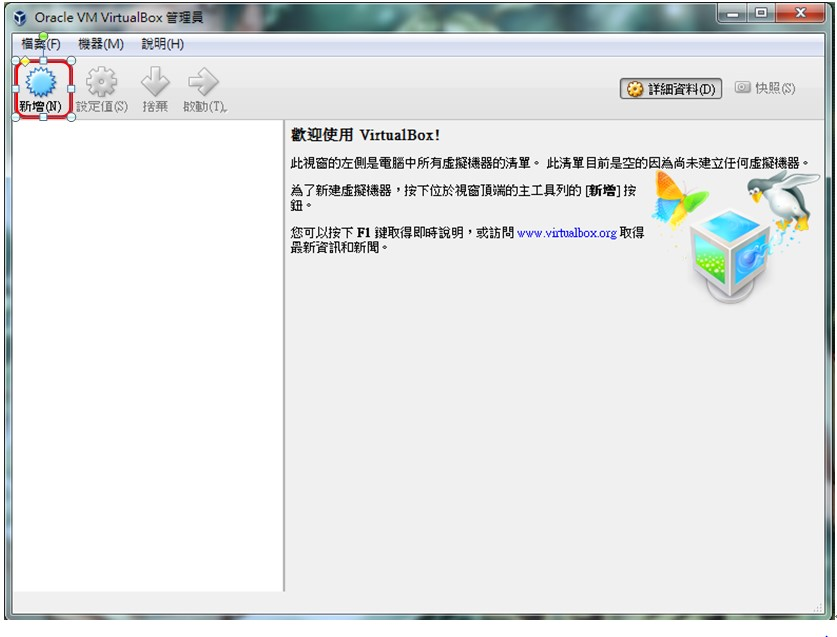
\includegraphics[width=300pt]{pic/圖片2.jpg}
    \end{center}
\end{figure}

\begin{figure}[htp]
    \begin{center}
        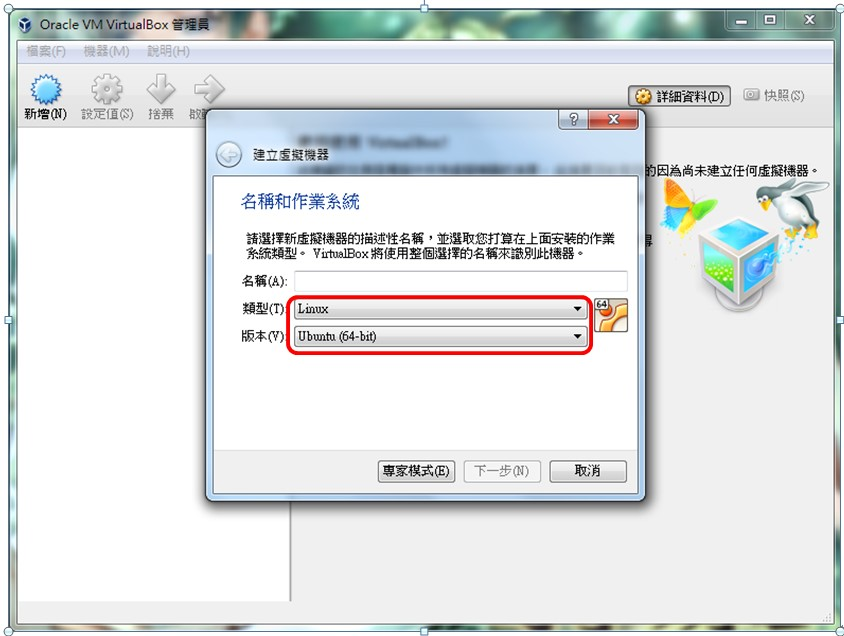
\includegraphics[width=300pt]{pic/圖片3.jpg}
    \end{center}
\end{figure}

\begin{figure}[htp]
    \begin{center}
        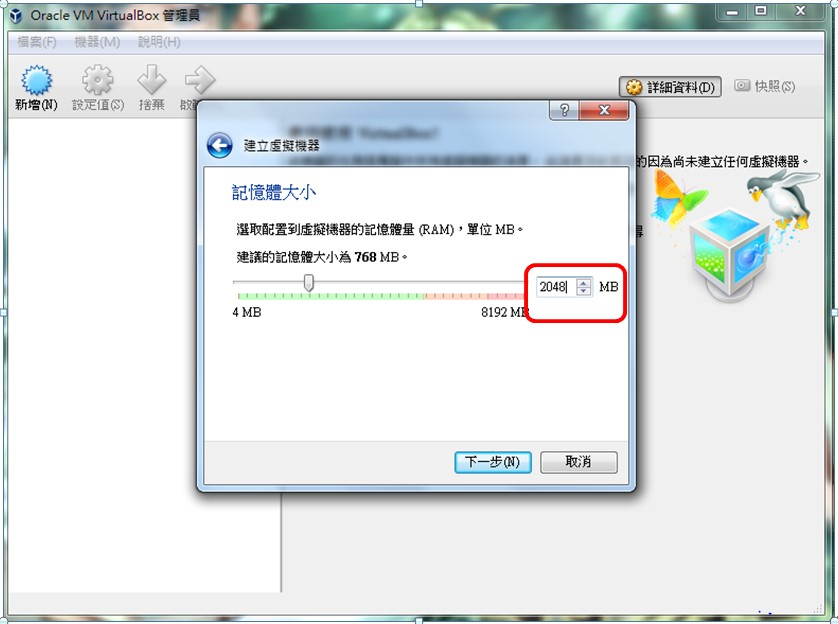
\includegraphics[width=300pt]{pic/圖片4.jpg}
    \end{center}
\end{figure}

\begin{figure}[htp]
    \begin{center}
        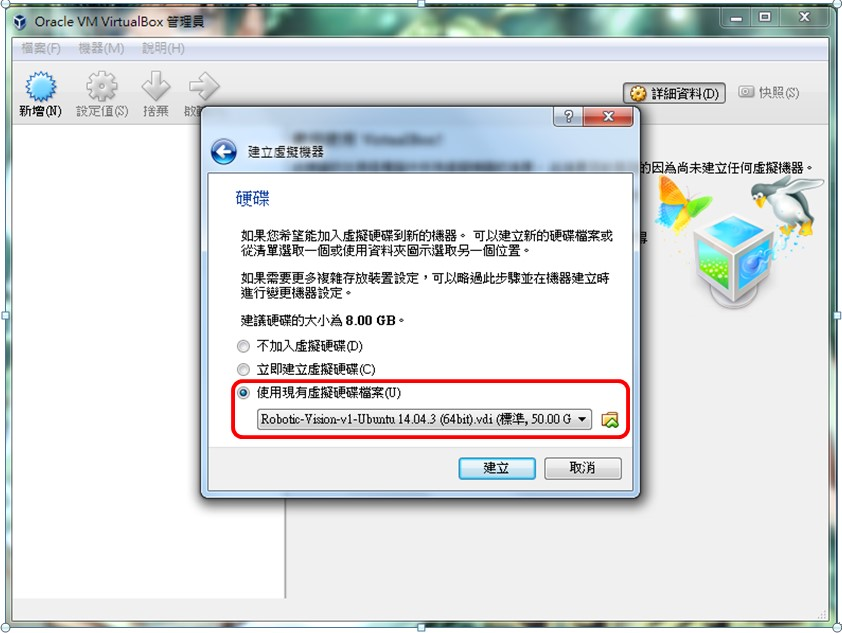
\includegraphics[width=300pt]{pic/圖片5.jpg}
    \end{center}
\end{figure}
\\
\\步驟四、VirtualBox網路設定
\\為了讓虛擬機器能連線到樹莓派,你需要沿著以下步驟去設定網路:
設定值 -> 網路 -> 橋接介面卡,當你使用公共網路若是無法使用橋接介面卡時,切換成NAT。

\begin{figure}[htp]
    \begin{center}
        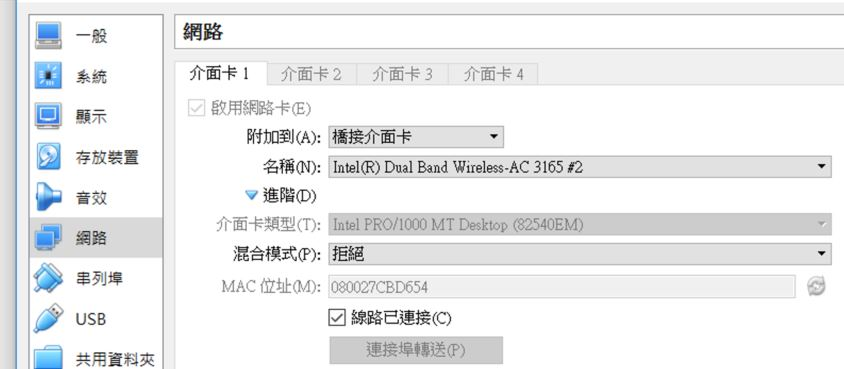
\includegraphics[width=300pt]{pic/圖片6.jpg}
    \end{center}
\end{figure}
\\步驟五、啟用Linux及剪貼簿設定
\begin{figure}[htp]
    \begin{center}
        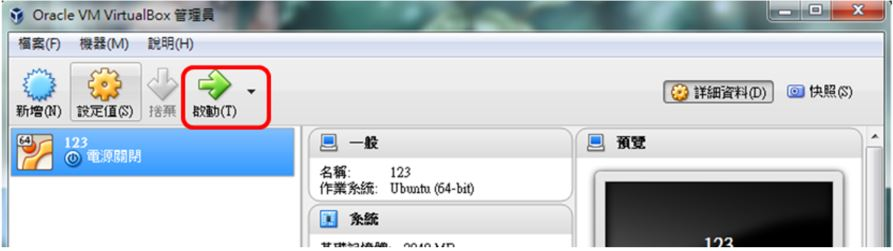
\includegraphics[width=300pt]{pic/圖片7.jpg}
    \end{center}
\end{figure}
\\Username/password > robotvision / assistiverobotics
\\啟動Linux後,開啟剪貼簿之雙向功能,以方便之後使用。
\begin{figure}[htp]
    \begin{center}
        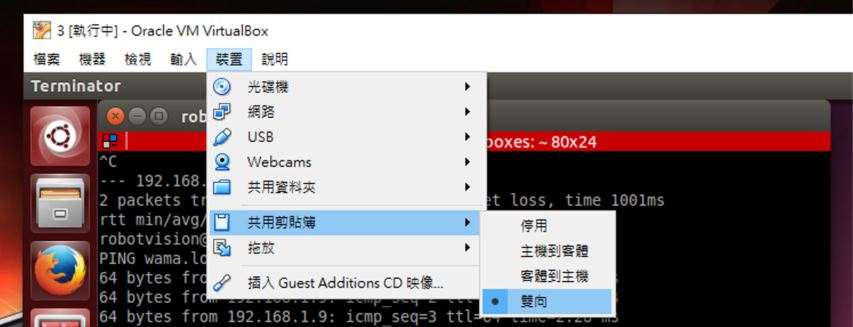
\includegraphics[width=300pt]{pic/圖片8.jpg}
    \end{center}
\end{figure}


\subsection{機器端網路設定}

網路設定方面,由於我們再進行程式編譯會以電腦進行遠端操作機器端上之程式撰寫、運作。主要以Wi-Fi路由器為溝通媒介,因此我們必須先確認機器端已經連線到Wi-Fi路由器上。
\begin{figure}[htp]
    \begin{center}
        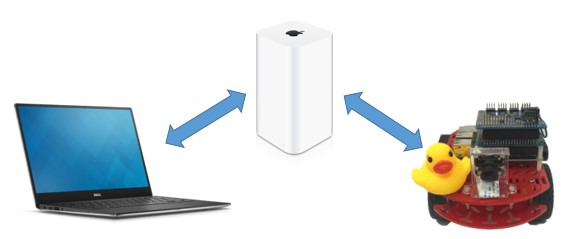
\includegraphics[width=300pt]{pic/圖片9.jpg}
    \end{center}
\end{figure}
\\先將機器以HDMI連接到外接螢幕並開啟電源,每一次更換無線網卡,都必須重複此步驟。
\\先確認網卡是否正常運作:
\\duckiebot \$ lsusb
\begin{figure}[htp]
    \begin{center}
        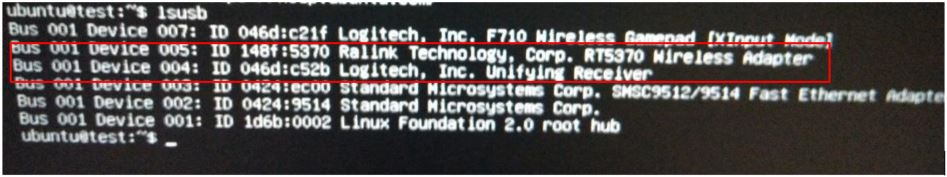
\includegraphics[width=300pt]{pic/圖片10.jpg}
    \end{center}
\end{figure}
\\接著,設定無線網路所連線之Wi-Fi路由器:
\\duckiebot \$ sudo vim /etc/wpa\_supplicant/wpa\_supplicant.conf
\begin{figure}[htp]
    \begin{center}
        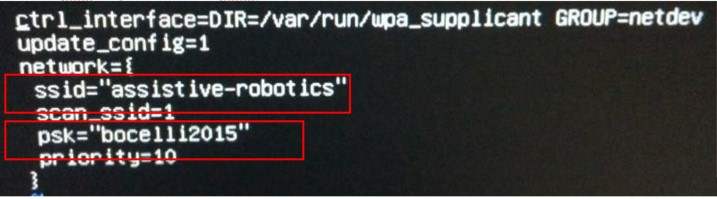
\includegraphics[width=300pt]{pic/圖片11.jpg}
    \end{center}
\end{figure}
\\根據你的Wi-Fi路由器更改以下兩行對應你的分享器
\\ssid="Wi-Fi帳號"
\\psk="Wi-Fi密碼"
\\修改完畢後,依步驟刪除70-persistent-net.rules再進行重啟:
\\duckiebot \$ sudo rm /etc/udev/rules.d/70-persistent-net.rules
\\duckiebot \$ sudo reboot
\\重啟完畢後,進行網路測試:
\\duckiebot \$ ping google.com
\begin{figure}[htp]
    \begin{center}
        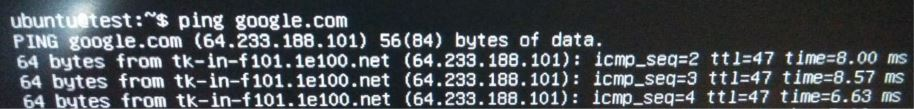
\includegraphics[width=300pt]{pic/圖片12.jpg}
    \end{center}
\end{figure}
\\如果你連上google,那就完成這個部份了。

\subsection{電腦端網路設定}

完成機器端之網路設定後,我們必須進行電腦端之網路設定。主要必須預留IP位址給予機器端,以確保每一次都能順利以電腦進行遠端操作。
\\
\\步驟一、紀錄機器端之MAC address
\\在機器端先進行IP設定之顯示:
\\duckiebot \$ ifconfig
\begin{figure}[htp]
    \begin{center}
        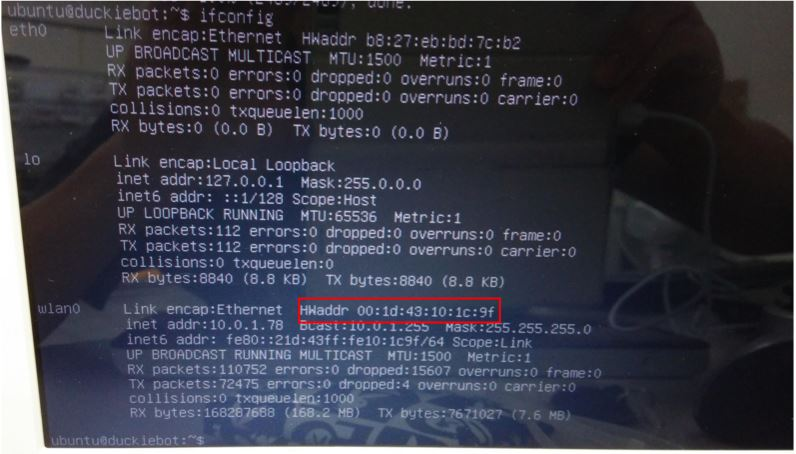
\includegraphics[width=300pt]{pic/圖片13.jpg}
    \end{center}
\end{figure}
\\此範例下,MAC address是“ 00:1d:43:10:1c:9f ”
\\
\\步驟二、進入Wi-Fi路由器設定介面
\\此範例中,我們使用的是TP-Link之路由器。不同之分享器有不同之IP。
\\打開一個瀏覽器輸入網址”192.168.0.254”,進行登入。
\\使用者名稱: admin   密碼: admin
\begin{figure}[htp]
    \begin{center}
        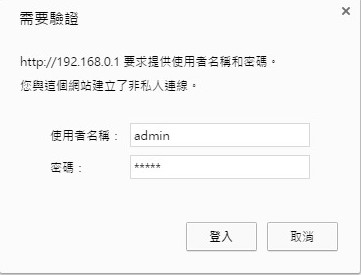
\includegraphics[width=300pt]{pic/圖片14.jpg}
    \end{center}
\end{figure}
\\
\\
\\
\\
\\步驟三、進行IP預留之設定
\\“進階設定” -> “DHCP” -> “位址保留” -> “新增”
\begin{figure}[htp]
    \begin{center}
        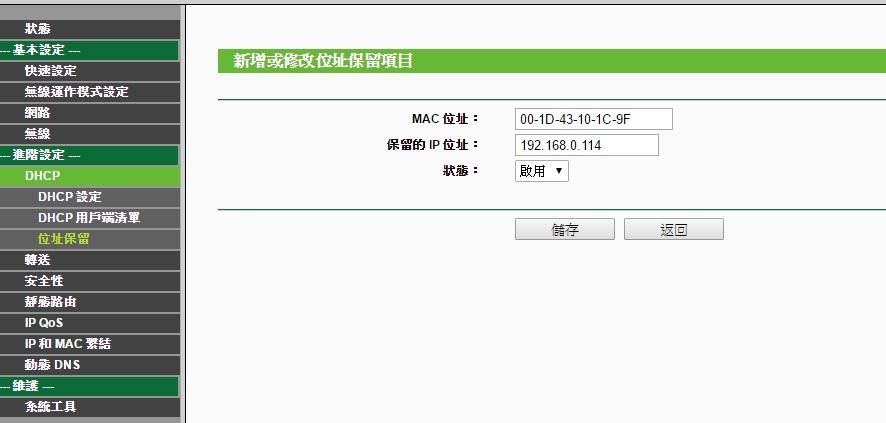
\includegraphics[width=300pt]{pic/圖片15.jpg}
    \end{center}
\end{figure}
\\MAC位址請填步驟一你紀錄之MAC address,IP之位址則為192.168.0.XXX,可依自己喜好設置,確保不要跟別其他裝置IP對沖。完成後儲存。
\\
\\步驟四、重啟Wi-Fi路由器及機器端
\\請手動重啟你的路由器,並同時重啟機器端:
\\duckiebot \$ sudo reboot

\section{程式環境架設}
在正式開始軟體部分前,我們必須先確定能透過Wi-Fi分享器以電腦端去對機器端進行遠端操作。首先先把機器端電源開啟並將電腦端Ubuntu開啟。

\subsection{遠端操作機器}
啟用Ubuntu後,我們須先將前一部分預留之機器端IP加到VirtualBox中:
\\\$ sudo vim /etc/hosts
\begin{figure}[htp]
    \begin{center}
        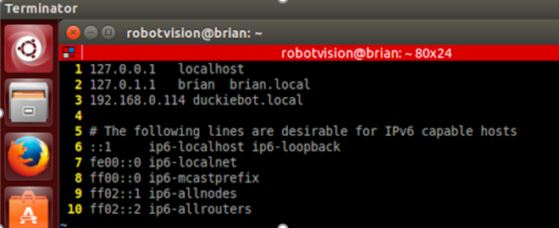
\includegraphics[width=300pt]{pic/圖片16.jpg}
    \end{center}
\end{figure}
\\在/etc/hosts中加上一行:192.168.0.XXX 你的車名.local
\\接下來,透過ssh來進行遠端操作:
\\\$ ssh ubuntu@your\_duckiebot.local     (此處your\_duckiebot為你的車名)
\\ssh是一個可以讓我們使用筆電遠端登入機器,並去操控機器執行指令

\subsection{程式環境掛載及彙編}

\section{ROS架構介紹及應用}
ROS又稱作為RobotOS,是專門為了機器人軟體開發所設計出的一套作業系統。他是一個開源的系統,任何人都可以在ROS上機器人相關之功能、系統。且其在系統間之溝通,是一個極為優秀之跨平台軟體通訊機制,藉由不同節點間之溝通去達到最佳效果。此外,在ROS本身就蘊含龐大的Library,其中不論是感測器資料、2或3D模擬介面、特定演算法資料庫等等,都廣為開放在ROS平台中。因此,使用者可以輕鬆地去使用其中之工具於研究之機器人平台上,並加以延伸應用。

\subsection{ROS架構解析}
在這一章節,將針對ROS中主要的各個運作項目作解釋。讓學生了解整體ROS是如何運作,各節點間如何溝通以及各個節點中之內容包含了哪些東西。
以下針對ROS架構中之各個項目進行分析,包含了Package、Node、Topic、Master、Messages、Parameter、Launch。
\\
\\ROS Package:
\\ROS Package的概念就是一個概括所有程式驅動、溝通橋樑及程式碼的集合體,是一個完整的程式組織。舉例來說,若今天要做一個人臉辨識之專題,所有的跑動程式碼、參數及相關之檔案都會放在一個名為Face Detection的Package裡。因此,在架構一個完整的系統時,必須建立一個屬於該系統之Package。ROS在建立Package上很容易,只需陸續在添入一些功能就好。
\\舉例來說,以下資料夾均為Duckietown中(catkin_ws/src)之 Package:

\begin{figure}[htp]
    \begin{center}
        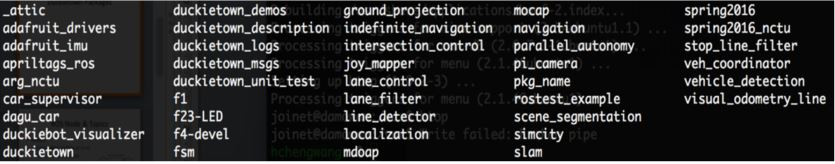
\includegraphics[width=300pt]{pic/圖片17.jpg}
    \end{center}
\end{figure}
\\ROS Node & Topic:
\\ROS Node在ROS中就是扮演著主要運行之核心程式碼的角色,每一個Node都是獨立運算之程式。Node一般可由C++或python構成,主要程式內容極為整個程式所使用到之功能、演算法等。而在不同的Node之間,Topic擔任資訊傳遞之角色。最主要是以Publish/Subscribe進行多個Node之間的訊息傳遞。在一個大系統中會概括許多個Node,而Topic即支援多對多之間的通訊。
\begin{figure}[htp]
    \begin{center}
        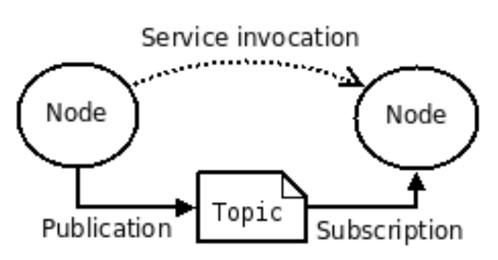
\includegraphics[width=300pt]{pic/圖片18.jpg}
    \end{center}
\end{figure}
\\舉例來說,Duckietown中每個Package也都概括許多Node:
\begin{figure}[htp]
    \begin{center}
        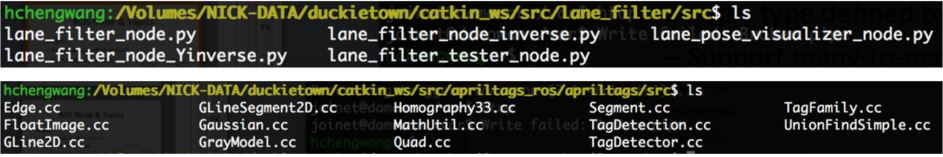
\includegraphics[width=300pt]{pic/圖片19.jpg}
    \end{center}
\end{figure}
\\
\\ROS Master:
\\在前面提到Node之間皆藉由Topic去進行訊息之傳遞,而Master則是負責管理所有Node之間的溝通。Master最大的功能就是將不同Node之間的Publisher與Subscriber以Topic進行連接,以確保他們的訊息能夠確實的連接起來。因此可知,Master主要是管理Node間該如何去做連接。
\begin{figure}[htp]
    \begin{center}
        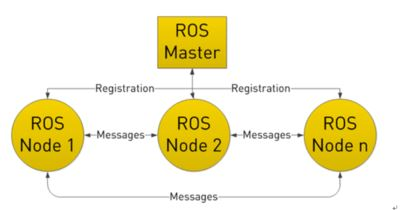
\includegraphics[width=300pt]{pic/圖片20.jpg}
    \end{center}
\end{figure}
\\而在多台Machine同時運作時,我們也可透過Master來進行多台Machine間之溝通。舉例來說,我們把機器與電腦都設成同樣的ROS Master,如此我們就可以進行機器與電腦之間的資訊傳遞。因此,在Duckietown運作前我們都會先把Master設定好,確保電腦與機器間能互相傳遞訊息。 
\\(舉例:\$ source set\_ros\_master.sh)
\begin{figure}[htp]
    \begin{center}
        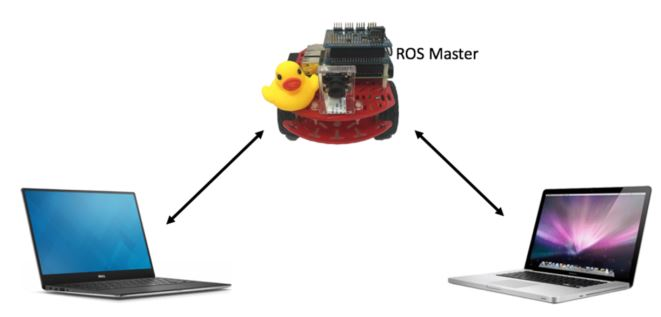
\includegraphics[width=300pt]{pic/圖片21.jpg}
    \end{center}
\end{figure}
\\ROS Message:
\\傳遞所用Topic之內容即為Message所構成及定義的,而不同的訊息傳遞也對應不同的type,像是bool, string, float32等等。Message就是溝通及傳遞之最基礎的訊息定義,Duckietown中之Message都以.msg檔案定義。
\begin{figure}[htp]
    \begin{center}
        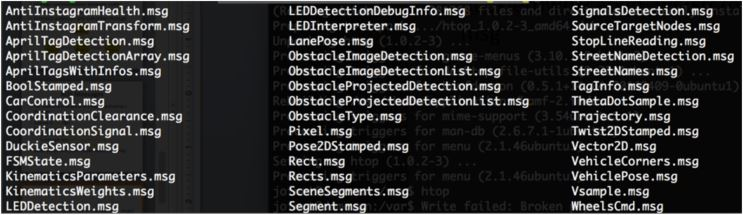
\includegraphics[width=300pt]{pic/圖片22.jpg}
    \end{center}
\end{figure}
\\
\\ROS Parameter:
\\每一個Node中之程式演算都一定會使用到特地功能之參數,譬如鏡頭畫素、馬達轉速等等。而在Duckietown中所有的參數檔都會統一歸類並放置duckietown/catkin\_ws/src/duckietown/config,以方便隨時替換參數值。
\\
\\ROS Launch:
\\Launch檔為XML檔,其主要功能是將Node組織化並定義好每個Node間之通訊及Parameter(參數)。當你啟動一個Launch時,他會啟用所有該檔中所定義的Node。是一個用來運作所有程式碼之工具,與驅動類似。而Duckietown中之Node都是依靠Launch來進行定義並運作的。

\begin{figure}[htp]
    \begin{center}
        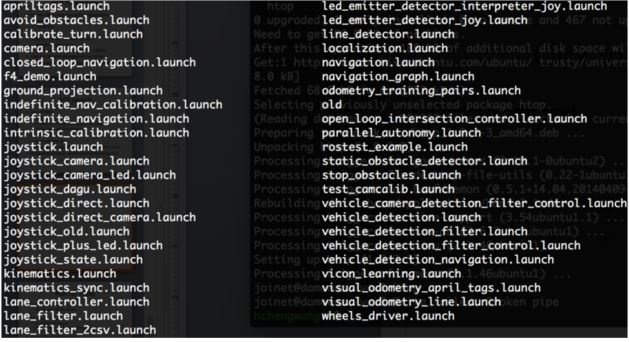
\includegraphics[width=300pt]{pic/圖片23.jpg}
    \end{center}
\end{figure}



\subsection{機器端之ROS應用}




\end{document}